
%% bare_conf.tex
%% V1.4b
%% 2015/08/26
%% by Michael Shell
%% See:
%% http://www.michaelshell.org/
%% for current contact information.
%%
%% This is a skeleton file demonstrating the use of IEEEtran.cls
%% (requires IEEEtran.cls version 1.8b or later) with an IEEE
%% conference paper.
%%
%% Support sites:
%% http://www.michaelshell.org/tex/ieeetran/
%% http://www.ctan.org/pkg/ieeetran
%% and
%% http://www.ieee.org/

%%*************************************************************************
%% Legal Notice:
%% This code is offered as-is without any warranty either expressed or
%% implied; without even the implied warranty of MERCHANTABILITY or
%% FITNESS FOR A PARTICULAR PURPOSE! 
%% User assumes all risk.
%% In no event shall the IEEE or any contributor to this code be liable for
%% any damages or losses, including, but not limited to, incidental,
%% consequential, or any other damages, resulting from the use or misuse
%% of any information contained here.
%%
%% All comments are the opinions of their respective authors and are not
%% necessarily endorsed by the IEEE.
%%
%% This work is distributed under the LaTeX Project Public License (LPPL)
%% ( http://www.latex-project.org/ ) version 1.3, and may be freely used,
%% distributed and modified. A copy of the LPPL, version 1.3, is included
%% in the base LaTeX documentation of all distributions of LaTeX released
%% 2003/12/01 or later.
%% Retain all contribution notices and credits.
%% ** Modified files should be clearly indicated as such, including  **
%% ** renaming them and changing author support contact information. **
%%*************************************************************************


% *** Authors should verify (and, if needed, correct) their LaTeX system  ***
% *** with the testflow diagnostic prior to trusting their LaTeX platform ***
% *** with production work. The IEEE's font choices and paper sizes can   ***
% *** trigger bugs that do not appear when using other class files.       ***                          ***
% The testflow support page is at:
% http://www.michaelshell.org/tex/testflow/



\documentclass[conference]{IEEEtran}
% Some Computer Society conferences also require the compsoc mode option,
% but others use the standard conference format.
%
% If IEEEtran.cls has not been installed into the LaTeX system files,
% manually specify the path to it like:
% \documentclass[conference]{../sty/IEEEtran}





% Some very useful LaTeX packages include:
% (uncomment the ones you want to load)


% *** MISC UTILITY PACKAGES ***
%
%\usepackage{ifpdf}
% Heiko Oberdiek's ifpdf.sty is very useful if you need conditional
% compilation based on whether the output is pdf or dvi.
% usage:
% \ifpdf
%   % pdf code
% \else
%   % dvi code
% \fi
% The latest version of ifpdf.sty can be obtained from:
% http://www.ctan.org/pkg/ifpdf
% Also, note that IEEEtran.cls V1.7 and later provides a builtin
% \ifCLASSINFOpdf conditional that works the same way.
% When switching from latex to pdflatex and vice-versa, the compiler may
% have to be run twice to clear warning/error messages.






% *** CITATION PACKAGES ***
%
%\usepackage{cite}
% cite.sty was written by Donald Arseneau
% V1.6 and later of IEEEtran pre-defines the format of the cite.sty package
% \cite{} output to follow that of the IEEE. Loading the cite package will
% result in citation numbers being automatically sorted and properly
% "compressed/ranged". e.g., [1], [9], [2], [7], [5], [6] without using
% cite.sty will become [1], [2], [5]--[7], [9] using cite.sty. cite.sty's
% \cite will automatically add leading space, if needed. Use cite.sty's
% noadjust option (cite.sty V3.8 and later) if you want to turn this off
% such as if a citation ever needs to be enclosed in parenthesis.
% cite.sty is already installed on most LaTeX systems. Be sure and use
% version 5.0 (2009-03-20) and later if using hyperref.sty.
% The latest version can be obtained at:
% http://www.ctan.org/pkg/cite
% The documentation is contained in the cite.sty file itself.






% *** GRAPHICS RELATED PACKAGES ***
%
\ifCLASSINFOpdf
  % \usepackage[pdftex]{graphicx}
  % declare the path(s) where your graphic files are
  % \graphicspath{{../pdf/}{../jpeg/}}
  % and their extensions so you won't have to specify these with
  % every instance of \includegraphics
  % \DeclareGraphicsExtensions{.pdf,.jpeg,.png}
\else
  % or other class option (dvipsone, dvipdf, if not using dvips). graphicx
  % will default to the driver specified in the system graphics.cfg if no
  % driver is specified.
  % \usepackage[dvips]{graphicx}
  % declare the path(s) where your graphic files are
  % \graphicspath{{../eps/}}
  % and their extensions so you won't have to specify these with
  % every instance of \includegraphics
  % \DeclareGraphicsExtensions{.eps}
\fi
% graphicx was written by David Carlisle and Sebastian Rahtz. It is
% required if you want graphics, photos, etc. graphicx.sty is already
% installed on most LaTeX systems. The latest version and documentation
% can be obtained at: 
% http://www.ctan.org/pkg/graphicx
% Another good source of documentation is "Using Imported Graphics in
% LaTeX2e" by Keith Reckdahl which can be found at:
% http://www.ctan.org/pkg/epslatex
%
% latex, and pdflatex in dvi mode, support graphics in encapsulated
% postscript (.eps) format. pdflatex in pdf mode supports graphics
% in .pdf, .jpeg, .png and .mps (metapost) formats. Users should ensure
% that all non-photo figures use a vector format (.eps, .pdf, .mps) and
% not a bitmapped formats (.jpeg, .png). The IEEE frowns on bitmapped formats
% which can result in "jaggedy"/blurry rendering of lines and letters as
% well as large increases in file sizes.
%
% You can find documentation about the pdfTeX application at:
% http://www.tug.org/applications/pdftex





% *** MATH PACKAGES ***
%
\usepackage{amssymb} %new add for \triangleq

\usepackage[cmex10]{amsmath}
%\usepackage{amsmath}
% A popular package from the American Mathematical Society that provides
% many useful and powerful commands for dealing with mathematics.
%
% Note that the amsmath package sets \interdisplaylinepenalty to 10000
% thus preventing page breaks from occurring within multiline equations. Use:
%\interdisplaylinepenalty=2500
% after loading amsmath to restore such page breaks as IEEEtran.cls normally
% does. amsmath.sty is already installed on most LaTeX systems. The latest
% version and documentation can be obtained at:
% http://www.ctan.org/pkg/amsmath





% *** SPECIALIZED LIST PACKAGES ***
%
\usepackage{algorithmic}
% algorithmic.sty was written by Peter Williams and Rogerio Brito.
% This package provides an algorithmic environment fo describing algorithms.
% You can use the algorithmic environment in-text or within a figure
% environment to provide for a floating algorithm. Do NOT use the algorithm
% floating environment provided by algorithm.sty (by the same authors) or
% algorithm2e.sty (by Christophe Fiorio) as the IEEE does not use dedicated
% algorithm float types and packages that provide these will not provide
% correct IEEE style captions. The latest version and documentation of
% algorithmic.sty can be obtained at:
% http://www.ctan.org/pkg/algorithms
% Also of interest may be the (relatively newer and more customizable)
% algorithmicx.sty package by Szasz Janos:
% http://www.ctan.org/pkg/algorithmicx




% *** ALIGNMENT PACKAGES ***
%
\usepackage{array}
% Frank Mittelbach's and David Carlisle's array.sty patches and improves
% the standard LaTeX2e array and tabular environments to provide better
% appearance and additional user controls. As the default LaTeX2e table
% generation code is lacking to the point of almost being broken with
% respect to the quality of the end results, all users are strongly
% advised to use an enhanced (at the very least that provided by array.sty)
% set of table tools. array.sty is already installed on most systems. The
% latest version and documentation can be obtained at:
% http://www.ctan.org/pkg/array


% IEEEtran contains the IEEEeqnarray family of commands that can be used to
% generate multiline equations as well as matrices, tables, etc., of high
% quality.




% *** SUBFIGURE PACKAGES ***
%\ifCLASSOPTIONcompsoc
%  \usepackage[caption=false,font=normalsize,labelfont=sf,textfont=sf]{subfig}
%\else
%  \usepackage[caption=false,font=footnotesize]{subfig}
%\fi
% subfig.sty, written by Steven Douglas Cochran, is the modern replacement
% for subfigure.sty, the latter of which is no longer maintained and is
% incompatible with some LaTeX packages including fixltx2e. However,
% subfig.sty requires and automatically loads Axel Sommerfeldt's caption.sty
% which will override IEEEtran.cls' handling of captions and this will result
% in non-IEEE style figure/table captions. To prevent this problem, be sure
% and invoke subfig.sty's "caption=false" package option (available since
% subfig.sty version 1.3, 2005/06/28) as this is will preserve IEEEtran.cls
% handling of captions.
% Note that the Computer Society format requires a larger sans serif font
% than the serif footnote size font used in traditional IEEE formatting
% and thus the need to invoke different subfig.sty package options depending
% on whether compsoc mode has been enabled.
%
% The latest version and documentation of subfig.sty can be obtained at:
% http://www.ctan.org/pkg/subfig




% *** FLOAT PACKAGES ***
%
%\usepackage{fixltx2e}
% fixltx2e, the successor to the earlier fix2col.sty, was written by
% Frank Mittelbach and David Carlisle. This package corrects a few problems
% in the LaTeX2e kernel, the most notable of which is that in current
% LaTeX2e releases, the ordering of single and double column floats is not
% guaranteed to be preserved. Thus, an unpatched LaTeX2e can allow a
% single column figure to be placed prior to an earlier double column
% figure.
% Be aware that LaTeX2e kernels dated 2015 and later have fixltx2e.sty's
% corrections already built into the system in which case a warning will
% be issued if an attempt is made to load fixltx2e.sty as it is no longer
% needed.
% The latest version and documentation can be found at:
% http://www.ctan.org/pkg/fixltx2e


%\usepackage{stfloats}
% stfloats.sty was written by Sigitas Tolusis. This package gives LaTeX2e
% the ability to do double column floats at the bottom of the page as well
% as the top. (e.g., "\begin{figure*}[!b]" is not normally possible in
% LaTeX2e). It also provides a command:
%\fnbelowfloat
% to enable the placement of footnotes below bottom floats (the standard
% LaTeX2e kernel puts them above bottom floats). This is an invasive package
% which rewrites many portions of the LaTeX2e float routines. It may not work
% with other packages that modify the LaTeX2e float routines. The latest
% version and documentation can be obtained at:
% http://www.ctan.org/pkg/stfloats
% Do not use the stfloats baselinefloat ability as the IEEE does not allow
% \baselineskip to stretch. Authors submitting work to the IEEE should note
% that the IEEE rarely uses double column equations and that authors should try
% to avoid such use. Do not be tempted to use the cuted.sty or midfloat.sty
% packages (also by Sigitas Tolusis) as the IEEE does not format its papers in
% such ways.
% Do not attempt to use stfloats with fixltx2e as they are incompatible.
% Instead, use Morten Hogholm'a dblfloatfix which combines the features
% of both fixltx2e and stfloats:
%
% \usepackage{dblfloatfix}
% The latest version can be found at:
% http://www.ctan.org/pkg/dblfloatfix




% *** PDF, URL AND HYPERLINK PACKAGES ***
%
%\usepackage{url}
% url.sty was written by Donald Arseneau. It provides better support for
% handling and breaking URLs. url.sty is already installed on most LaTeX
% systems. The latest version and documentation can be obtained at:
% http://www.ctan.org/pkg/url
% Basically, \url{my_url_here}.




% *** Do not adjust lengths that control margins, column widths, etc. ***
% *** Do not use packages that alter fonts (such as pslatex).         ***
% There should be no need to do such things with IEEEtran.cls V1.6 and later.
% (Unless specifically asked to do so by the journal or conference you plan
% to submit to, of course. )

\ifCLASSOPTIONcompsoc
\usepackage[caption=false,font=normalsize,labelfon
t=sf,textfont=sf]{subfig} \else
\usepackage[caption=false,font=footnotesize]{subfi
g} \fi
\usepackage{mdwmath}
\usepackage{mdwtab}
\usepackage{multirow}
\usepackage[ruled,vlined]{algorithm2e}
\usepackage{graphicx}
\usepackage{epstopdf}

\newcommand{\figwidth}{0.75\linewidth}
\newcommand{\figwidthsmall}{0.5\linewidth}
\newcommand{\figwidtha}{0.7\linewidth}
\newcommand{\figwidthb}{0.80\linewidth}
\newcommand{\figwidthdouble}{0.5\linewidth}
\newcommand{\figwidthtriple}{0.32\linewidth}
\def\figref#1{Fig.~\ref{#1}}
\def\secref#1{Section~\ref{#1}}
\def\tabref#1{Table~\ref{#1}}
%\DeclareMathOperator{\sgn}{sgn}
%\DeclareMathOperator{\num}{num}
%\DeclareMathOperator{\erf}{erf}
%\DeclareMathOperator{\mean}{mean}
%\DeclareMathOperator{\Cov}{Cov}
%\DeclareMathOperator{\E}{E}
%\DeclareMathOperator{\Var}{Var}
\DeclareMathOperator{\trace}{trace}
%\DeclareMathOperator{\tr}{tr}

% correct bad hyphenation here
\hyphenation{op-tical net-works semi-conduc-tor}


\begin{document}
%
% paper title
% Titles are generally capitalized except for words such as a, an, and, as,
% at, but, by, for, in, nor, of, on, or, the, to and up, which are usually
% not capitalized unless they are the first or last word of the title.
% Linebreaks \\ can be used within to get better formatting as desired.
% Do not put math or special symbols in the title.
\title{End-to-end pipeline for ground truth generation, video annotation and evaluation of object detection models}
%Improved Video Annotation and Modelling tool

% author names and affiliations
% use a multiple column layout for up to three different
% affiliations
%\author{\IEEEauthorblockN{Michael Shell}
%\IEEEauthorblockA{School of Electrical and\\Computer Engineering\\
%Georgia Institute of Technology\\
%Atlanta, Georgia 30332--0250\\
%Email: http://www.michaelshell.org/contact.html}
%\and
%\IEEEauthorblockN{Homer Simpson}
%\IEEEauthorblockA{Twentieth Century Fox\\
%Springfield, USA\\
%Email: homer@thesimpsons.com}
%\and
%\IEEEauthorblockN{James Kirk\\ and Montgomery Scott}
%\IEEEauthorblockA{Starfleet Academy\\
%San Francisco, California 96678--2391\\
%Telephone: (800) 555--1212\\
%Fax: (888) 555--1212}}


 \author{\IEEEauthorblockN{Unnikrishnan Kizhakkemadam Sreekumar, Qi Li, Revathy Devaraj, Kaikai Liu}
 \IEEEauthorblockA{Computer Engineering Department\\
 San Jose State University (SJSU)\\
 San Jose, CA, USA
 Email: \{unnikrishnan.kizhakkemadamsreekumar, qi.li, revathy.devaraj, kaikai.liu\}@sjsu.edu}
 }
 
% conference papers do not typically use \thanks and this command
% is locked out in conference mode. If really needed, such as for
% the acknowledgment of grants, issue a \IEEEoverridecommandlockouts
% after \documentclass

% for over three affiliations, or if they all won't fit within the width
% of the page, use this alternative format:
% 
%\author{\IEEEauthorblockN{Michael Shell\IEEEauthorrefmark{1},
%Homer Simpson\IEEEauthorrefmark{2},
%James Kirk\IEEEauthorrefmark{3}, 
%Montgomery Scott\IEEEauthorrefmark{3} and
%Eldon Tyrell\IEEEauthorrefmark{4}}
%\IEEEauthorblockA{\IEEEauthorrefmark{1}School of Electrical and Computer Engineering\\
%Georgia Institute of Technology,
%Atlanta, Georgia 30332--0250\\ Email: see http://www.michaelshell.org/contact.html}
%\IEEEauthorblockA{\IEEEauthorrefmark{2}Twentieth Century Fox, Springfield, USA\\
%Email: homer@thesimpsons.com}
%\IEEEauthorblockA{\IEEEauthorrefmark{3}Starfleet Academy, San Francisco, California 96678-2391\\
%Telephone: (800) 555--1212, Fax: (888) 555--1212}
%\IEEEauthorblockA{\IEEEauthorrefmark{4}Tyrell Inc., 123 Replicant Street, Los Angeles, California 90210--4321}}




% use for special paper notices
%\IEEEspecialpapernotice{(Invited Paper)}




% make the title area
\maketitle

% As a general rule, do not put math, special symbols or citations
% in the abstract
\begin{abstract}
Video annotation as a means to gather ground truth is proven to be beneficial in the progress of machine learning(ML) and deep learning(DL) techniques like object detection and classification. 
To develop such learning models or to re-train existing models, researchers and developers heavily rely on ground truth dataset to train their neural-networks(NN). 
The process of generating ground truth from video sequences, most of the time, requires large amount of manual effort. 
Today, to develop a product with Artificial Intelligence (AI), there is no framework that guides through the process of selecting a viable model. 
In the cycle of AI enabled application development, fast ground truth generation and model selection are closely connected tasks which could be worked on together. 
With this paper, we propose an user friendly front-end tool that supports semi-automated video annotation to generate ground truth with considerably less manual effort, especially focussing on the object-classes a product developer could choose. 
In addition to supporting semi-automated ground truth generation, the tool provides interface for high level model evaluation. 
Such an evaluation, with the proposed system, guides the developer to visually compare and analyse the performance of two or more models. 
The main contribution of this paper is to show a detailed methodology to perform the closely connected tasks of fast dataset generation, testing and evaluation of extant models. 
Obtained results suggest that such a system will drastically reduce the cost associated with AI application development. 
\end{abstract}

% no keywords
\begin{IEEEkeywords}
Semi-Automated Video annotation, model evaluation metrics, multi-model interactive auto-annotation tool, ground truth generation.
\end{IEEEkeywords}

% For peer review papers, you can put extra information on the cover
% page as needed:
% \ifCLASSOPTIONpeerreview
% \begin{center} \bfseries EDICS Category: 3-BBND \end{center}
% \fi
%
% For peerreview papers, this IEEEtran command inserts a page break and
% creates the second title. It will be ignored for other modes.
\IEEEpeerreviewmaketitle


\section{Introduction}

With this paper, we propose three major advents:
1) The automatic ground truth (GT) generation capability, for the classes specifically asked for by the user. The tool proposed in the paper is mainly for deep neural network based object detection and classification models.
2) An easy way to plug in any object detection and classification model from the long, ever growing list of such exciting new models. s
3) Evaluate the performance of these models on the decided list of classes on a high level. The evaluation metric we use are highly precise and take care of evaluating the predicted output against the GT.

The proposed system, is called IVADL (Improved Video Annotation and more for Deep Learning).

1) Automatic GT generation is not something new. \cite{dominguez2014gtgencv} explains a similar methodology of generating semi-automated GT which reduces human intervention and thus resulting in faster GT generation. Papers like \cite{comaschi2014gtgencv} and \cite{kavasidis2012gtgencv} also explored ways to generate accurate GT by using Computer Vision algorithms to detect contours and objects. The use of "the wisdom of the crowd" (\cite{dominguez2014gtgencv}) to derive the best results from the outputs of multiple Computer Vision algorithms excited us. We decided to give an auto-annotation feature where the system run precision tests between multiple predictions on the same frame to come up with the GT decision as derived from multiple object-detection models. \par
Unlike the extant systems addressing GT generation, the system proposed in this paper utilises neural networks. Also, the system as such is meant to generate ground truth for the classes a particular application developer would desire. When generating GT, there are multiple aspects to care about. Some of those attributes are:
a) accurate bounding boxes around the object.
b) exact classification information.
c) object ID as tracked between frames in a video or an image-list.

2) The system proposes a generic, yet simple programming interface to plugin object detection models. The model shall implement the API with:
a) A function that defines all the classes of interest, input video or image-list. This defines the interface to invoke a model.
b) A callback function that has to be implemented within the purview of the model wherein each predicted object is represented as a bounding box (BB).
c) The API interface defines the data structures in a way that any model could inherently include an object tracking mechanism or rely on IVADL's object tracking mechanism where in BB's from multiple frames are tracked with a unique BB identifier (BBID).

With the above two modules of the proposed system, we shall be able to generate GT in a very limited time for humongous input data videos or image lists. After the interim-GT generation, the proposed system gives the human user a easy-to-use Graphical User Interface (GUI) to easily correct BB's classification confidence and tracking confidence aspects. Such corrected GT are the key information helping researchers in the field to solve real-world problems. 

Most of the existing solutions, like NVIDIA DIGITS, that allow models to be plugged in depends on a broad programming interface defined by a framework, like Caffe, tensorflow or darknet. The proposed interface is as simple as the two functions discussed above enabling developers to easily plugin a number of models into IVADL. These models in-turn could be an open-source evaluation wrapped with one of the frameworks. 

3) Now, with an established GT produced with the desired list of classes, a developer would wish to quickly compare multiple models (those used for interim-GT generation and probably more) against the final GT. The proposed system uses state of the art evaluation criteria similar to the techniques discussed in \cite{everingham2010vocchallenge} to generate a comprehensive evaluation report that can be visualised in an improved easy-to-understand GUI.
The GUI shall include individual sections describing the evaluation results of each model. These sections are divided into two main compartments:
a) The report to be visualised per frame.
\begin{itemize}
	\item A video player playing back the video or list of images on which the objects are detected. The object detection output, namely the BB's shall be coloured in a way the developer can easily make out the correctness of each of the BB's.
	\item A graph visualiser which would be in sync with the above video area. The graph plots evaluation report for each frame.
	\item Class specific statistical data elements denoting precision and accuracy of detections per frame shall be displayed in a tabular form.
\end{itemize}
b) The report to be visualised for the entire video or image-list.
\begin{itemize}
	\item A graph visualiser which would plot the evaluation report for the entire video or image-list.
	\item Class specific statistical data elements denoting precision and accuracy for all the detections in the video or image-list shall be displayed in a tabular form.
\end{itemize}
The GUI shall be explained in detail in the following sections.

Such an interactive multi-model video annotation tool where one can select model(s), auto-annotate objects, evaluate the results, visualise the performance metrics and work on rapid prototyping of application is the holy grail of neural-network based application development and research.\par
The system keeps track of the evaluation metric in terms of object classification accuracy, bounding box precision and undetected objects that are manually added. This evaluation metric could even help the researcher to easily track weak spots and improve on the learning algorithm. The comprehensive evaluation module integrates easy to understand representation of pitfalls, accuracy measures and errors on a per class, per frame, per video basis. \par
The system discussed in this paper is developed as part of a research project aimed at creating an ecosystem that supports easy ground truth generation, model evaluation and application development. The tool helps developers to quickly generate ground truth for classes of interest, evaluate available DNN models for those classes. \par
In order to reduce the annotation work for the worker, BeaverDam uses interpolation to annotate a video between two manually annotated frames. Although this approach lowers the complexity for the worker, the accuracy for bounding boxes are not guaranteed and the interpolated results are discarded during the process. In this paper, we will present a new approach to generate the annotated bounding boxes automatically with high precision.\par
Furthermore, the system discussed in this paper supports labelling and learning an infinite number of classes.  \par

\section{Proposed System}\label{sec.overview}

\subsection{Motivation}

\subsection{System Architecture}
The Integrated Video Annotation for Deep Learning (IVADL) tool is a web application built on the existing Beaver Dam Video annotation tool [1] . The proposed system consists of three major components: (i) A server and the database with the evaluation engine (ii) The Client Interface(CI) with an easy-to-use User Interface(UI) to display the annotation and evaluation results (iii) The Model Interface(MI) that connects the pre-trained classification models used for auto-annotation. Fig [1]  describes the architecture of the proposed system with each module described in detail in the preceding sub-sections. 

\begin{figure}[htb]
\centering
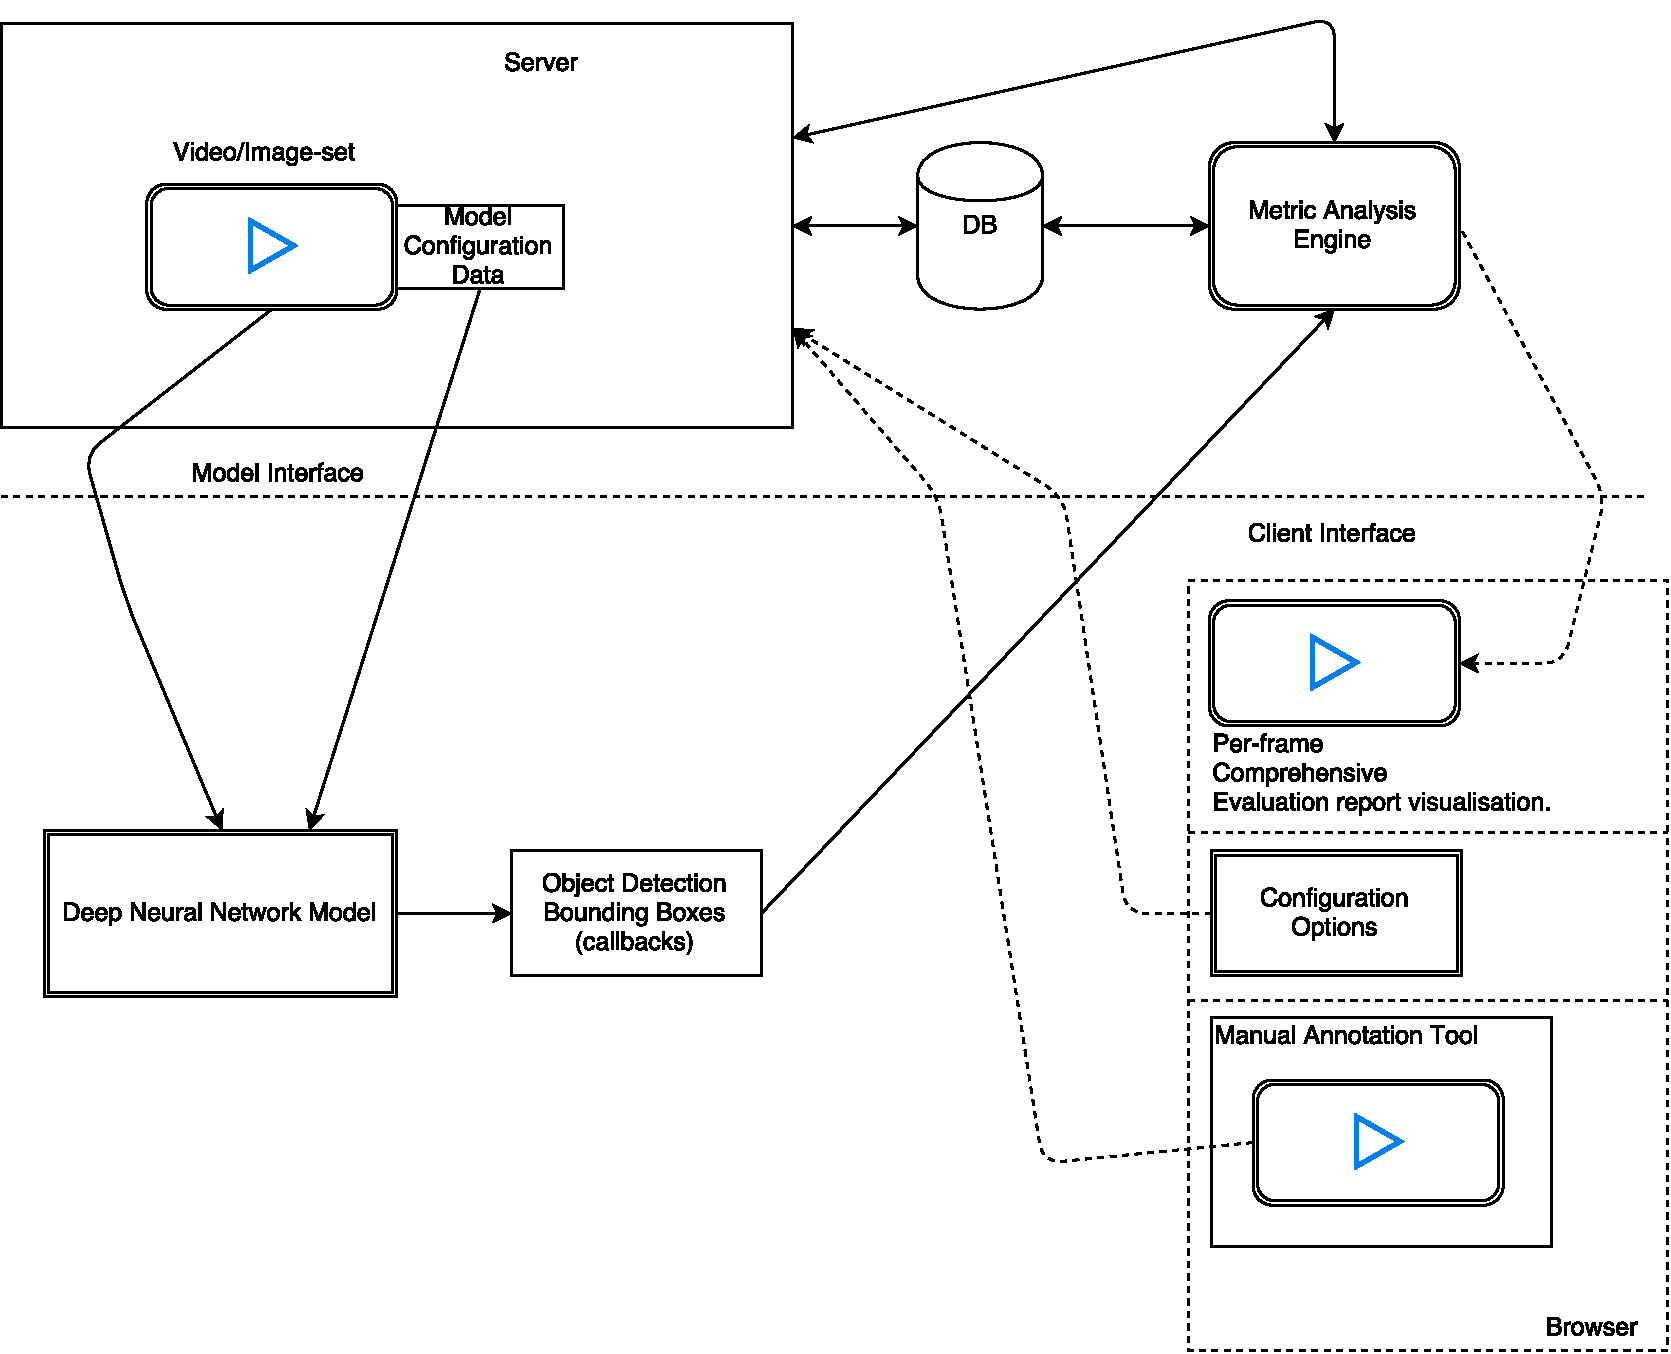
\includegraphics[width=\figwidthb]{fig/system_architecture.pdf}
\caption{System Architecture.} \label{fig.structure}
\end{figure}

\subsubsection{Server}
The back-end of the system is the Server hosting  the  video/image-set database in [? where to deploy the web app]. The server module could be hosted on a CUDA enabled server, like the NVIDIA DGX. It implements basic video annotation features like managing user-account, retrieving annotation data, evaluating the metrics, presenting the results and managing the classification label. There can be administrator users and staff users. Administrator will be able to add/delete users, video annotation jobs, classification labels for annotation. Staff users will be able to view the video annotation jobs and annotate appropriately the objects identified under the list of provided labels.
\subsubsection{Model interface (MI)}
The classifier models are the core component of the auto-annotation system. With a view to make the system flexible, application programming interface (API) is provided as a part of the system to add/remove models, select from multiple models, compare the  evaluation results between selected models. This design provides two major functionality (i) Allows user to select among various classifier algorithms based on its performance (ii)  Allows user to  to run the new models for evaluation of its metrics.[details about API ??] . The system by default is integrated with two popular models (i) YOLO [2] , darknet based model (ii) Fast RCNN [3] , tensorflow based model. Section 3.2 describes these selected models.
\subsubsection{Metric analysis engine (MAE)}
The metric analysis engine is a part of server that performs high-level evaluation of the annotation results and models performance metrics[1].  The evaluation methodology is based on the PASCAL VOC 2009 Challenge [4] and the techniques that are used to detect accuracy counts [5] is based on paper[6]. In addition it supports filtered list of user selected classifiers for evaluation of its metrics. The tuning parameters such as IoU ratio threshold, confidence score of a prediction are user configurable. The MAE shall evaluate the following metrics:
(i) Bounding box confidence score and precision (ii)Accuracy count of the model inference (iii) F1 score,Precision and Recall values for all the classifiers (iv) Average precision and Mean Average precision of a classifier model.These metrics and its evaluation are presented graphically in a table or graph format by MAE as shown below. 
\subsubsection{Client interface (CI)}
The client interface is a web browser where it shall render the user interfaces for: (i) Manual correction of video annotation (ii) Selection and configuration of classifier model (iii) running auto-annotation (iv) view comprehensive evaluation report. The precision of all bounding boxes are color coded to visually represent the values. The UI supports list of labels that can be auto-annotated by the models and enables user to filter the labels to view and evaluate those classes. The evaluation summary view presents the data for each model selected for evaluation with the video play option to support per frame evaluation. 


\section{Methodology}
\subsection{Annotation Method} \label{sec.annotation}
In order to perform auto-annotation of the video sequence on real-time basis, we propose to use the state-of-art real-time object detection systems with high-accuracy. Two such models we chose to integrate to IVADL tool by default are YOLO9000 [1] and FAST RCNN [2]. [add details about these models, labels, training details, dataset used]. These models support the frame level and sequence level object detection and classification. The technique we propose for ground truth generation is to first run the model on the entire video to generate the predicted list of objects by the model and do manual correction of the predicted list to generate the final ground truth for the given data-set. This ground truth data is then used for the evaluation of each of the object classifiers and compare the relative performance of those models. \par

Let F = \textit{ f1, f2, f3,.., fn}  be the video sequence with n frames Let P =  \textit{p1, p2, p3,..., pn}  be the predicted  object list for corresponding frames of F, generated by the classifier model. Let BB be the set of bounding boxes that represent the classified objects in F and  for each object let bbx =  \textit{x, y, w, h, f, t} where  x ,y is  X co-ordinate and Y co-ordinate of the starting point of a bounding box, w is width of the bounding box, h is height of the bounding  box, f is the frame id where the bounding box is located, t is the tracker flag updated by the object tracking model . On running the selected classifier models on F, initial ground truth list P is generated.Currently the system we propose employs manual correction of P to generate G, where G is the final ground truth with the highest accuracy that is to be used for evaluation of other models integrated to the system. \par

Along with annotation of objects, we propose to use object tracking models to correlate the predicted bounding boxes of each frame in F. [add details about object tracker]. After generating G, the result of the annotation phase on running model 1 is P1 object list, for model 2 is P2 object list.

\subsection{Evaluation Method} \label{sec.evaluation}
The evaluation of P1,P2 objects list described in section \ref{sec.annotation} are based on the method used by PASCAL VOC09 challenge evaluation [1]. According to PASCAL VOC evaluation[1] three accuracy metrics are computed to evaluate a multi-class models (i) Precision-Recall values with different rank cutoff (ii) Average precision representing the area of Precision-Recall curve (iii) mean average precision for all the classes in a multi-class model. Prior to the computation of above listed accuracy metrics, the predicted objects and its bounding boxes are verified against the ground truth objects by calculating its IoU (Intersection of Union) and the computation details are explained in the following subsection.
\subsubsection{IoU} \label{ref.iou}
We use IoU for 2 purposes (i) Mapping the bounding boxes \textit{bbx} between predicted object list and ground truth object list (ii) bounding box precision is evaluated using IoU where the threshold for IoU is a tunable parameter set by the user. By calculating IoU for each \textit{bbx} in G with all  \textit{bbx} in P, the pair with max IoU value is mapped with same bounding box ID. Let  A$_{\text{g}}$ be the area of ground truth bounding box, A{$_{\text{p}}$} be the area of predicted bounding box, then IoU is calculated using the formula below.
\begin{align}
{IoU}= \frac {A_g \cap  A_p} {A_g \cup A_p}
\end{align}
\begin{align}
{bbID_g,_p} = {max ( IoU ( bbx_g , \forall  bbx_p ))}
\end{align}
\subsubsection{Accuracy Metrics} \label{ref.accuracy}
The common evaluation metrics for classification models has 4 basic accuracy counts[1] (i) True Positive (ii) True negatives (iii) False Positive (iv) False negatives, that is used to find the precision and recall values as mentioned above. These metrics are calculated for each class/label of the multi-class model.In the system we propose, we support calculation of these metrics on frame by frame basis and for complete video sequence. Let t{$_{\text{p}}$} be true positive that represent the number of objects classified correctly, f{$_{\text{p}}$} be false positive that is the number of objects classified in-correctly in the predicted list.  Let t{$_{\text{n}}$} be true positive that represent the number of objects not classified correctly, f{$_{\text{n}}$} be false negative that is the number of objects not classified in-correctly in the predicted list. The precision indicates the percentage of true positives in the classified objects' list and recall is a measure of the percentage of objects correctly classified.
\begin{align}
{Precision}= \frac {t_p} {t_p + f_p}
\end{align}
\begin{align}
{Recall}= \frac {t_p} {t_p + f_n}
\end{align}
\subsubsection{Precision Recall Graph for each class}
The performance of a model is denoted by numerical value called Average precision of a class in a multi-class model. A model is considered good if its with high precision and recall values measured for different ranks values. Thus the area under precision-recall curve represents models performance and it is plotted between the precision and recall values of a class across the frame or video for different subsets of predicted output, giving us a pretty good visualization of the model quality. The subset used here is sampled from the list of classified bounding boxes, sorted with the model's rank. Popular evaluation models like the one used with VOC Challenge[1] uses a 11-point sampling, but we propose the more accurate k-point sampling, where we plot precision-recall values for every subset that results a change in the recall metric.
	$${AP} = \sum_{k=1}^{N} P(k) {\Delta}r(k)$$
\subsubsection{Mean Average Precision}
	Mean average precision, {mAP} is the mean of the {AP} values calculated for each of the classes supported by the multi-class model. This measure is a single-valued metric used to compare the models performance. Model with high value of {mAP} is the desired one used for application. The evaluation results enables the user to compare different models and select the model for a specific application. This system thus provides the user mechanism for rapid ground truth generation and model selection.The evaluation metrics are displayed in the below table format,
\begin{align}
\begin{tabular}{| c | c | c | c | c | c | c | }
\hline
Model & Class (CAR) & & & & & Classes \\ 
\hline 
     & tp & tn & fp & fn & AP & mAP \\ 
YOLO & 769 & 0 &  108 & 56 & 0.89 & 0.19  \\
FRCNN & 723 & 0 & 3 & 5 & 0.99 & 0.974 \\
\hline
\end{tabular}
\end{align}




\section{Experiments} \label{sec.experiment}
\subsection{Data} \label{sec.data}
\subsection{Results} \label{sec.results}
\begin{figure}
\centering
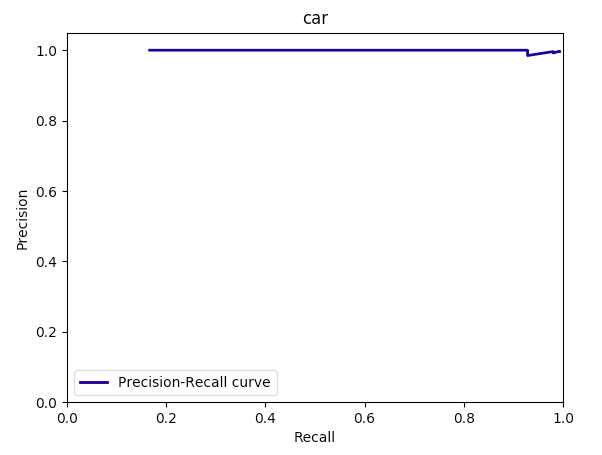
\includegraphics[width=\figwidthb]{fig/pr_rcnn.png}
\caption{Prediction recall curve when we ran RCNN, class "Car" for a 2 second video.} \label{fig.structure}
\end{figure}

\begin{figure}
\centering
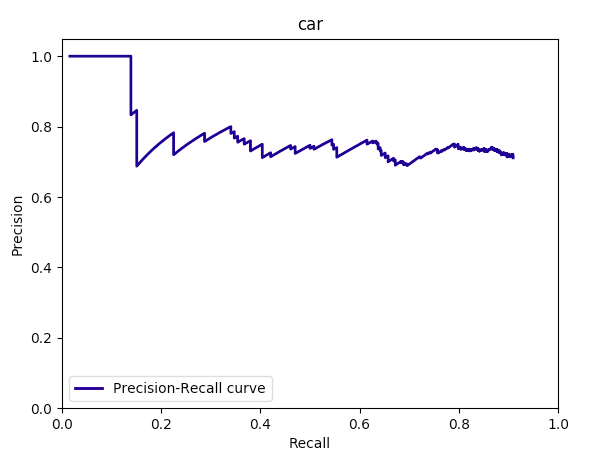
\includegraphics[width=\figwidthb]{fig/pr_yolo.png}
\caption{Prediction recall curve when we ran YOLO, class "Car" for a 2 second video.} \label{fig.structure}
\end{figure}

\subsection{Average Precision for each class}
	Average precision is the single number derived from the above graph, simply by taking the area under the plotted curve.
	$${AP} = \int_{0}^{1} P(r) dr$$
	Practically the area under the curve could be implemented as:
	$${AP} = \sum_{k=1}^{N} P(k) {\Delta}r(k)$$
\subsection{Interpolated Average Precision for each class}
	Interpolated average precision is calculated the same way as we calculated {AP} above, but, instead of using {P(k)}, the maximum precision value: 
	$${max}_{k\textsuperscript{'}>= k} {P(k\textsuperscript{'})}$$
	Thus:
	$${IAP} = \sum_{k=1}^{N} {max}_{k\textsuperscript{'}>= k} {P(k\textsuperscript{'})} {\Delta}r(k)$$

\subsection{Mean Average Precision across all the classes the model was trained on}
	Mean average precision, {mAP} is the mean of the {AP} values calculated for each of the classes supported by the model. 

\subsection{Future Work}




%\begin{figure}
%\centering
%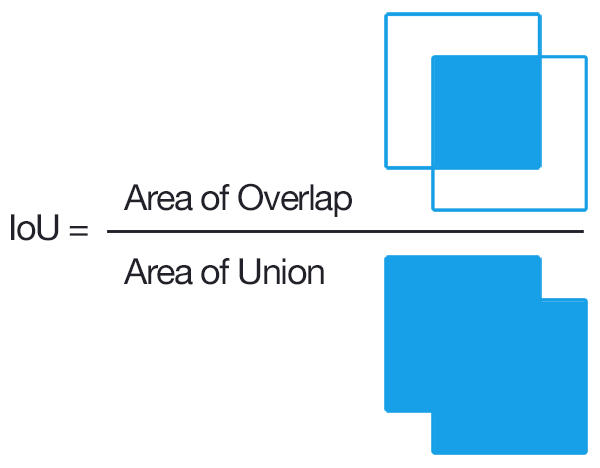
\includegraphics[width=\figwidthb]{fig/iou_equation.png}
%\caption{IoU equation.} \label{fig.structure}
%\end{figure}

	
%Math symbol: $\hat{r}_{n,m}^{(k)}$.

%Equations:
%\begin{align}
%\mathbf{f}_t^n=\mathbf{R}_b^n \mathbf{f}_t^b + \mathbf{e}^n
%\end{align}
%where $\mathbf{e}^n$ is the error of the force that applied to the smartphone. The figure is shown in \figref{fig.doublefigure} and \figref{fig.structure}.

%\begin{figure}[htb]
%\centerline{\subfloat[Figure 1]{\includegraphics[width
%=0.5\linewidth]{fig/city.pdf} \label{fig.figure1}} \hfil
%\subfloat[Figure 2]{\includegraphics[width=0.5\linewidth]{fig/city.pdf}
%\label{fig.figure2}}
%} \caption{The figure for: (a) Figure1; (b) Figure2.} \label{fig.doublefigure}
%\end{figure}






\section{Related Work}\label{sec.related}

There is a significant amount of image and video data that researchers wish to utilise efficiently. However, without properly label or annotate, the data will become waste. Therefore, developing annotation tools for different purposes is almost as important as these large datasets themselves.

For image annotation, Abhishek Dutta, Ankush Gupta and Andrew Zisserman of the Visual Geometry Group of University of Oxford developed a simple browser-based tool, which supports region shapes of rectangle, circle, ellipse, polygon and point, called VGG Image Annotator (VIA)\cite{abh2017via}, which can be utilised offline with json format output. NVIDIA AI City Challenge 2017 used DMIAT as its annotation platform. Torralba et al(2010)\cite{Russell2008labelme} proposed a LabelMe tool for static image annotation.  

However, the static image annotation tools do not have the capabilities to handle the continuous nature of the video. Consequently there is significant effort in developing annotation tools for video datasets. Ching-Yung et al(2003)\cite{lin2003videoann} developed VideoAnnEx MPEG-7 Annotation Tool. Yuen J, Russell B, Liu C, Torralba A (2009)\cite{yuen2009labelmevideo} introduced LabelMe Video, an open web-based platform can generate event annotations. Carl V, Donald P, Deva R\cite{carl2012vatic} described Video Annotation Tool from Irvine, California (VATIC). Mihalcik D, Doermann D (2003) presented ViPER\cite{mihalcik2003viper}, a local based software for spatial labeling. Anting S\cite{shen2016beaverdam} described BeaverDam, an easy-installed browser-based tool. In order to lower the annotation cost, Ali et al (2011)\cite{ali2011flowboost} present a method that can populate labels and annotations for a video with only few keyframes annotated. BeaverDam and LabelMe Video use linear interpolation. Agarwala et al (2004)\cite{agarwala2004tracker} describe that by using trackers, object tracking between keyframes would be more precise and more appropriate in rotoscoping and animation. I. Kavasidis et al(2012)\cite{I2012GTTool} presented GTTool which uses Snakes\cite{kass1988snakes} (not polygons), Gaussian Mixture Model (GMM)\cite{stauffer1999gmm} and CAMSHIFT\cite{bradski1998camshift} to generate ground truth automatically. Ground Truth Verification Tool (GTVT)\cite{ambardekar2009gtvt} for video surveillance systems uses simple blob tracking\cite{gupte2002sblobtrack} and calculate the accuracy of bounding boxes.

Considering the cost of annotating large volume visual datasets and the limitations of individual worker, tools for annotation is not enough. Ching-Yung et al(2003)\cite{lin2003videoann} proposed the Video Collaboration Annotation Forum as a corporation effort to annotate TRECVID\cite{smeaton2006trecvid} 2003 video set via the VideoAnnEx MPEG-7 Annotation Tool. A. Sorokin and D. Forsyth introduced Amazon Mechanical Turk(AMT)\cite{sorokin2008amt} for labeling vision data. ImageNet\cite{deng2009imgnet} dataset used AMT to clean its candidate images. VATIC and BeaverDam also have AMT interface built in. 

For the Deep Learning purpose, we further developed BeaverDam, combined the evaluation concepts of Pascal VOC challenge\cite{everingham2010vocchallenge}, and created a unique browser-based, user-based, end to end video annotation tool, which integrated with object detection models to reduce the annotation workload.

The need for having an end-to-end pipeline for DNN modelling and training has been tackled by the project named DIGITS. NVIDIA provides DIGITS under the BSD license, available at http://github.com/NVIDIA/DIGITS. The essential difference between DIGITS and the system proposed in this paper is the fact that our system attempts to closely integrate data-set generation techniques like video annotation and modelling together. This substantially mitigate the ordeal involved with training and modelling of deep neural networks.

There are some projects discussing the process of automatically annotating videos using deep learning like \cite{baptist2016automatedendtoend}, with a focus on multimedia archive search-ability. 

\section{Conclusion}\label{sec.conclusion}


% conference papers do not normally have an appendix


% use section* for acknowledgment
%\section*{Acknowledgment}


%The authors would like to thank...





% trigger a \newpage just before the given reference
% number - used to balance the columns on the last page
% adjust value as needed - may need to be readjusted if
% the document is modified later
%\IEEEtriggeratref{8}
% The "triggered" command can be changed if desired:
%\IEEEtriggercmd{\enlargethispage{-5in}}

% references section

% can use a bibliography generated by BibTeX as a .bbl file
% BibTeX documentation can be easily obtained at:
% http://mirror.ctan.org/biblio/bibtex/contrib/doc/
% The IEEEtran BibTeX style support page is at:
% http://www.michaelshell.org/tex/ieeetran/bibtex/
%\bibliographystyle{IEEEtran}
% argument is your BibTeX string definitions and bibliography database(s)
%\bibliography{IEEEabrv,../bib/paper}
%
% <OR> manually copy in the resultant .bbl file
% set second argument of \begin to the number of references
% (used to reserve space for the reference number labels box)

%\bibliographystyle{IEEEtran}
%\bibliography{IEEEmybib}

%\begin{thebibliography}{1}
%
%\bibitem{IEEEhowto:kopka}
%H.~Kopka and P.~W. Daly, \emph{A Guide to \LaTeX}, 3rd~ed.\hskip 1em plus
%  0.5em minus 0.4em\relax Harlow, England: Addison-Wesley, 1999.
%
%\end{thebibliography}

\begin{thebibliography}{9}

\bibitem{baptist2016automatedendtoend} 
B. Vandersmissen et al., "An Automated End-To-End Pipeline for Fine-Grained Video Annotation using Deep Neural Networks," in 
\textit{International Multimedia Conference.}, Amsterdam, 2016, pp.409-412.
 
\bibitem{redmon2016yolo9000} 
J. Redmon and A. Farhadi. (2016, December 25). 
\textit{YOLO9000: Better, Faster, Stronger} (\textit{2nd ed.}) [Online]. Available: https://arxiv.org/abs/1612.08242

\bibitem{vondrick2011vatic}
C. Vondrick et al., "Efficiently Scaling Up Crowdsourced Video Annotation", \textit{International Journal of Computer Vision.}, pp. 0920-5691, June. 2012.

\bibitem{everingham2010vocchallenge}
M. Everingham et al., "The Pascal Visual Object Classes (VOC) Challenge", \textit{International Journal of Computer Vision.}, vol.88, no.2, pp. 303-338, June. 2010.

\bibitem{doennann2000ViPER} 
D. Doennann and D. Mihalcik, "Tools and techniques for video performance evaluation," in 
\textit{Pattern Recognition, 2000. Proceedings. 15th International Conference.}, Barcelona, 2000, pp.167-170. doi: 10.1109/ICPR.2000.902888
    
\bibitem{shen2016beaverdam} 
A. Shen, "BeaverDam: Video Annotation Tool for Computer Vision Training Labels," M.S. thesis, EECS, Univ. California, Berkeley, CA, 2016.

\bibitem{abh2017via}
VGG Image Annotator : Visual Geometry Group. (2017, July 22). Retrieved from http://www.robots.ox.ac.uk/~vgg/software/via/

\bibitem{Russell2008labelme}
B. C. Russell, A. Torralba, K. P. Murphy, and W. T. Freeman, ?Labelme: A database and web-based tool for image annotation,? Int. J. Comput. Vision, vol. 77, no. 1-3, pp. 157?173, May 2008.

\bibitem{lin2003videoann}
C. Lin and B. Tseng, ?Video collaborative annotation forum: Establishing ground-truth labels on large multimedia datasets,? Proceedings of the TRECVID 2003, 2003

\bibitem{yuen2009labelmevideo}
Yuen J, Russell B, Liu C, Torralba A (2009) LabelMe video: Building a Video Database with Human Annotations. International Conference of Computer Vision

\bibitem{carl2012vatic}
Carl Vondrick, Donald Patterson, Deva Ramanan. "Efficiently Scaling Up
Crowdsourced Video Annotation" International Journal of Computer Vision
(IJCV). June 2012.(VATIC)

\bibitem{mihalcik2003viper}
Mihalcik D, Doermann D (2003) The Design and Implementation of ViPER. Technical Report 

\bibitem{ali2011flowboost}
Ali K, Hasler D, Fleuret F (2011) Flowboost? appearance learning from sparsely annotated video. IEEE Computer Vision and Pattern Recognition 

\bibitem{agarwala2004tracker}
Agarwala A, Hertzmann A, Salesin D, Seitz S (2004) Keyframe-based tracking for rotoscoping and animation. In: ACM Transactions on Graphics (TOG), ACM, vol 23, pp 584?591

\bibitem{I2012GTTool}
I. Kavasidis, S. Palazzo, R. Di Salvo, D. Giordano, C. Spampinato (2012), ?A semi-automatic tool for detection and tracking ground truth generation in videos,? Proceedings of the 1st International Workshop on Visual Interfaces for Ground Truth Collection in Computer Vision Applications - VIGTA '12 - 2012

\bibitem{kass1988snakes}
M. Kass, A. Witkin, and D. Terzopoulos, ?Snakes: Active contour models,? International Journal of Computer Vision, vol. 1, no. 4, pp. 321?331, Jan. 1988.	

\bibitem{stauffer1999gmm}
C. Stauffer and W. E. L. Grimson, ?Adaptive background mixture models for real-time tracking,? Computer Vision and Pattern Recognition, IEEE Computer Society Conference on, vol. 2, pp. 246?252, 1999.

\bibitem{bradski1998camshift}
G. R. Bradski, ?Computer Vision Face Tracking For Use in a Perceptual User Interface,? Intel Technology Journal, pp. 1?15, 1998.

\bibitem{ambardekar2009gtvt}
A. Ambardekar and M. Nicolescu, ?Ground Truth Verification Tool (GTVT) for Video Surveillance Systems,? in Advances in Computer-Human Interactions, 2009. ACHI ?09. Second International Conferences on, Cancun, 2009, pp. 354?359.	

\bibitem{gupte2002sblobtrack}
S. Gupte, O. Masoud, R. F. K. Martin, and N. P. Papanikolopoulos, ?Detection and Classification of Vehicles,? IEEE Transactions on Intelligent Transportation Systems, vol. 3, no. 1, pp. 37-47, 2002. 

\bibitem{smeaton2006trecvid}
Smeaton A, Over P, Kraaij W (2006) Evaluation campaigns and trecvid. In: Proceedings of the 8th ACM international workshop on Multimedia information retrieval, ACM, pp 321?330

\bibitem{sorokin2008amt}
A. Sorokin and D. Forsyth. Utility data annotation with amazon mechanical turk. In InterNet08, pages 1?8, 2008.

\bibitem{deng2009imgnet}
J. Deng, W. Dong, R. Socher, L.-J. Li, K. Li, and L. Fei-Fei, ?ImageNet: A Large-Scale Hierarchical Image Database,? in CVPR09, 2009.

\bibitem{dominguez2014gtgencv}
G. F. Dominguez, "Semi-automatic Generation of Accurate Ground Truth Data in Video Sequences," in 
\textit{2014 International Conference on Advances in Computing, Communications and Informatics.}, New Delhi, 2014, pp. 310-315. doi: 10.1109/ICACCI.2014.6968309

\bibitem{kavasidis2012gtgencv}
I. Kavasidis, "A Semi-automatic Tool for Detection and Tracking Ground Truth Generation in Videos," in \textit{Proceedings of the 1st International Workshop on Visual Interfaces for Ground Truth Collection in Computer Vision Applications.}, Capri, 2012, pp. 1-5. doi: 10.1145/2304496.2304502

\bibitem{comaschi2014gtgencv}
F. Comaschi et al., "A tool for fast ground truth generation for object detection and tracking from video," in \textit{IEEE International Conference on Image Processing (ICIP)}, Paris, 2014, pp. 368-372. doi: 10.1109/ICIP.2014.7025073


\end{thebibliography}
% that's all folks
\end{document}


